\documentclass{article}
\usepackage{graphicx}
\usepackage{amssymb}
\usepackage{amsmath}
\usepackage[margin=1in]{geometry}
\usepackage{float}
\usepackage{color}

\newcommand{\rd}{\mathrm{d}}
\newcommand{\eps}{\varepsilon}
\newcommand{\Lap}{\mathcal{L}}
\newcommand{\Res}{\operatorname*{Res}}

\title{Derivation of the Analytic Solution of the Coupled DL--AL Problem\\
via the Time--Laplace / Resolvent Construction}
\author{Kevin Bedoya \and (analysis notes)}
\date{June 2026}

\begin{document}

\maketitle

\begin{abstract}
The product ansatz $F=R(r)\Theta(\theta)$ and the additive ansatz
$F=A(r)+B(r)\Theta(\theta)$ both fail to produce an exact single--$\sigma$
eigenmode of the coupled diffusive--layer (DL) / advective--layer (AL) operator;
the failure is structural (the operator is non--self--adjoint, and two angular
channels demand incompatible Bessel--zero spectra). The correct construction is
therefore not an eigenfunction expansion but a \emph{resolvent} one: Laplace
transform in time, solve the resulting modified--Helmholtz boundary value problem
in closed form, and recover the decay rates as the poles of the resolvent. This
note carries that program through end to end. We (1) transform the system and
eliminate the AL density exactly; (2) represent the microtubule (MT) sources on
the full disk through a Dirac comb, which feeds every angular harmonic and
resolves the cusp paradox; (3) build the per--mode radial Green's function in
closed modified--Bessel form; (4) close the problem into a single Fredholm
integral equation whose secular determinant $\det(\mathcal I+\mathcal A(s))=0$
furnishes the (generally complex) decay rates; (5) invert by the Bromwich
contour to obtain $\phi(r,\theta,t)$ and $\rho(r,t)$ as residue series --- the
analytic solution; and (6) evaluate the leading two--mode truncation explicitly,
reproducing the numerically observed $g(r)+a(r)\cos N\theta$ structure.
\end{abstract}

\section{The system and the strategy}

On the disk $r\in[0,1]$ with $N$ evenly spaced microtubules along the rays
$\theta_i=2\pi i/N$, the densities $\phi$ (DL) and $\rho_i$ (AL) obey
\begin{align}
\partial_t\phi &=\nabla^2\phi
+\sum_{i}\frac1r\bigl(b\,\rho_i(r,t)-a\,\phi(r,\theta_i,t)\bigr)\delta(\theta-\theta_i),
\label{eq:phi}\\
\partial_t\rho_i &= v\,\partial_r\rho_i + a\,\phi(r,\theta_i,t)-b\,\rho_i(r,t),
\label{eq:rho}
\end{align}
with absorbing conditions $\phi(1,\theta,t)=0$, $\rho_i(1,t)=0$, the
angularly symmetric initial data $\phi(r,\theta,0)=\phi_0(r)$,
$\rho_i(r,0)=0$. By the $N$--fold symmetry all $\rho_i$ are equal
($\rho_i\equiv\rho$) and $\phi(r,\theta_i,t)$ is the same on every ray; we use the
representative ray $\theta=0$.

\paragraph{Why Laplace, not eigenfunctions.} The operator is not self--adjoint:
the advection $v\,\partial_r$ and the one--sided MT coupling break symmetry, so a
real discrete spectrum with a complete orthogonal eigenbasis is not guaranteed,
and indeed (companion notes) no separated eigenmode exists. The robust route is
to solve the initial value problem by Laplace transform,
\begin{equation}
\widehat g(\,\cdot\,,s)=\int_0^\infty e^{-st}\,g(\,\cdot\,,t)\,\rd t,
\end{equation}
in which the decay rates appear as the \emph{poles} of the resolvent
$\widehat\phi(r,\theta,s)$ in the complex $s$--plane. The full time response is
then reconstructed by contour integration. This is exact and makes no
separability assumption.

\section{Laplace transform and exact AL elimination}

Transforming \eqref{eq:phi}--\eqref{eq:rho} and using the initial data,
\begin{align}
(\nabla^2-s)\,\widehat\phi &= -\phi_0(r)
-\sum_i\frac1r\bigl(b\,\widehat\rho-a\,\widehat\phi(r,0,s)\bigr)\delta(\theta-\theta_i),
\label{eq:phihat}\\
v\,\partial_r\widehat\rho-(s+b)\,\widehat\rho &= -a\,\widehat\phi(r,0,s),
\qquad \widehat\rho(1,s)=0 .
\label{eq:rhohat}
\end{align}
Equation \eqref{eq:rhohat} is first order in $r$; with the integrating factor
$e^{-\frac{s+b}{v}r}$ and the terminal condition $\widehat\rho(1)=0$,
\begin{equation}
\boxed{\;
\widehat\rho(r,s)=-\frac{a}{v}\,e^{\frac{s+b}{v}r}
\int_1^r e^{-\frac{s+b}{v}r'}\,\psi(r',s)\,\rd r'
\;=:\;\mathcal R[\psi](r,s),
\qquad
\psi(r,s):=\widehat\phi(r,0,s).
\;}
\label{eq:Rfunctional}
\end{equation}
The AL density is thus a known \emph{linear functional} of the DL trace
$\psi=\widehat\phi(\cdot,0,s)$ on the MT ray. (This is the $\sigma\to-s$ image of
the elimination used in the problem statement.) Substituting \eqref{eq:Rfunctional}
into the source of \eqref{eq:phihat} closes the problem on $\widehat\phi$ alone:
the MT source on each ray is
\begin{equation}
\frac{1}{r}\,q(r,s),\qquad
q(r,s):=b\,\mathcal R[\psi](r,s)-a\,\psi(r,s),
\label{eq:qdef}
\end{equation}
a linear functional of $\psi$.

\section{Disk representation: the Dirac comb feeds every harmonic}

The comb of MT rays has the Fourier representation
\begin{equation}
\sum_{i=0}^{N-1}\delta(\theta-\theta_i)
=\frac{N}{2\pi}\sum_{n\in\mathbb Z}e^{inN\theta},
\label{eq:comb}
\end{equation}
since $\sum_{i=0}^{N-1}e^{-im\theta_i}=N$ when $N\mid m$ and $0$ otherwise. Hence
\eqref{eq:phihat} becomes
\begin{equation}
(\nabla^2-s)\,\widehat\phi
=-\phi_0(r)+\frac{N}{2\pi}\,\frac{q(r,s)}{r}\sum_{n\in\mathbb Z}e^{inN\theta}.
\label{eq:phihat2}
\end{equation}
Expanding $\widehat\phi(r,\theta,s)=\sum_{n\in\mathbb Z}\widehat\phi_n(r,s)\,e^{inN\theta}$
and matching harmonics gives, for each $n$, an inhomogeneous radial equation
\begin{equation}
\Lap_{nN}\widehat\phi_n:=
\widehat\phi_n''+\frac1r\widehat\phi_n'
-\Bigl(s+\frac{(nN)^2}{r^2}\Bigr)\widehat\phi_n
=-\phi_0(r)\,\delta_{n0}+\frac{N}{2\pi}\,\frac{q(r,s)}{r},
\label{eq:moderad}
\end{equation}
with $\widehat\phi_n(1,s)=0$ and regularity at $r=0$.

\paragraph{Resolution of the cusp paradox.} A naive Fourier--in--$\theta$
treatment on a single wedge makes the MT condition look like an over--counted
``third'' boundary condition (companion audit note). On the full disk the comb
\eqref{eq:comb} shows the true mechanism: the MT source $q(r,s)/r$ enters the
\emph{right--hand side of every} mode equation \eqref{eq:moderad}, with equal
weight $N/2\pi$. The derivative cusp at each ray is encoded by this common
forcing across all orders $nN$ --- not by any single smooth harmonic. Every
$\widehat\phi_n$ is therefore sourced and nonzero, and the modes are coupled
through the single scalar functional $q$.

\section{The per-mode radial Green's function}

Write \eqref{eq:moderad} in Sturm--Liouville form by multiplying by $r$:
$\frac{\rd}{\rd r}\!\bigl(r\,\widehat\phi_n'\bigr)-\bigl(sr+\tfrac{(nN)^2}{r}\bigr)\widehat\phi_n=r\,(\text{RHS})$.
The homogeneous solutions of $\Lap_m u=0$ are the modified Bessel functions
$I_m(\sqrt s\,r)$ (regular at $0$) and $K_m(\sqrt s\,r)$ (singular at $0$).
Construct
\begin{equation}
u_1(r)=I_m(\sqrt s\,r),\qquad
u_2(r)=K_m(\sqrt s)\,I_m(\sqrt s\,r)-I_m(\sqrt s)\,K_m(\sqrt s\,r),
\end{equation}
so that $u_1$ is regular at the origin and $u_2(1)=0$ enforces the absorbing
condition. Their Abel constant follows from the modified--Bessel Wronskian
$I_m'(z)K_m(z)-I_m(z)K_m'(z)=1/z$:
\begin{equation}
p(r)\bigl[u_1u_2'-u_1'u_2\bigr]
=r\cdot\sqrt s\,I_m(\sqrt s)\,
\bigl[I_m'(z)K_m(z)-I_m(z)K_m'(z)\bigr]_{z=\sqrt s r}
=I_m(\sqrt s)\quad(\text{const}).
\end{equation}
The (positive) Green's kernel for $\Lap_m u=F\Rightarrow u(r)=-\int_0^1 r'\,\mathcal K_m(r,r';s)\,F(r')\,\rd r'$ is therefore
\begin{equation}
\boxed{\;
\mathcal K_m(r,r';s)=
\frac{I_m(\sqrt s\,r_<)}{I_m(\sqrt s)}
\Bigl[I_m(\sqrt s)\,K_m(\sqrt s\,r_>)-K_m(\sqrt s)\,I_m(\sqrt s\,r_>)\Bigr],
\;}
\label{eq:Kgreen}
\end{equation}
with $r_<=\min(r,r')$, $r_>=\max(r,r')$. By construction $\mathcal K_m(r,1;s)=0$
and $\mathcal K_m$ is regular at $r=0$. Note the poles of \eqref{eq:Kgreen} in $s$
sit at the zeros of $I_m(\sqrt s)$, i.e.\ at $s=-\kappa_{mN,j}^2$ (since
$I_m(\sqrt s)=0\Leftrightarrow J_m(\sqrt{-s})=0$): these are precisely the
\emph{uncoupled} ($a=b=0$) Dirichlet decay rates. The MT coupling will move them.

\paragraph{Forced ($n=0$) response.} With $F=-\phi_0$ for $n=0$,
\begin{equation}
\Phi_0(r,s):=\int_0^1 r'\,\mathcal K_0(r,r';s)\,\phi_0(r')\,\rd r' .
\label{eq:Phi0}
\end{equation}
For a central $\delta$--release $\phi_0(r)=\delta(r)/(2\pi r)$ (unit mass in 2D),
$r_<=0$, $I_0(0)=1$, and \eqref{eq:Phi0} collapses to the explicit closed form
\begin{equation}
\Phi_0(r,s)=\frac{1}{2\pi}
\Bigl[K_0(\sqrt s\,r)-\frac{K_0(\sqrt s)}{I_0(\sqrt s)}\,I_0(\sqrt s\,r)\Bigr].
\label{eq:Phi0delta}
\end{equation}

\paragraph{MT--sourced part (all $n$).} With $F=\frac{N}{2\pi}q/r$,
\begin{equation}
\widehat\phi_n(r,s)=\delta_{n0}\,\Phi_0(r,s)
-\frac{N}{2\pi}\int_0^1 \mathcal K_{nN}(r,r';s)\,q(r',s)\,\rd r' .
\label{eq:phin}
\end{equation}

\section{Closing the system: Fredholm equation and secular determinant}

Evaluate \eqref{eq:phin} on the MT ray $\theta=0$, where $e^{inN\cdot 0}=1$, and
sum over $n$:
\begin{equation}
\psi(r,s)=\widehat\phi(r,0,s)=\sum_n\widehat\phi_n(r,s)
=\Phi_0(r,s)-\int_0^1 \mathcal S(r,r';s)\,q(r',s)\,\rd r',
\label{eq:psieq}
\end{equation}
where the rays--summed kernel
\begin{equation}
\mathcal S(r,r';s):=\frac{N}{2\pi}\sum_{n\in\mathbb Z}\mathcal K_{nN}(r,r';s)
\label{eq:Skernel}
\end{equation}
is the Dirichlet Green's function of $(\nabla^2-s)$ on the disk, restricted to a
common ray and summed over the $N$--fold comb (by the addition theorem
$\sum_n I_n K_n e^{in\Delta\theta}$ it is the image--corrected
$\tfrac{1}{2\pi}K_0(\sqrt s|\mathbf r-\mathbf r'|)$ on the rays; we keep it as
\eqref{eq:Skernel}). Insert the closure \eqref{eq:qdef},
$q=b\,\mathcal R[\psi]-a\,\psi$, into \eqref{eq:psieq}:
\begin{equation}
\boxed{\;
\psi(r,s)+\int_0^1 \mathcal S(r,r';s)
\bigl(b\,\mathcal R[\psi](r',s)-a\,\psi(r',s)\bigr)\rd r'
=\Phi_0(r,s).
\;}
\label{eq:fredholm}
\end{equation}
This is a linear Fredholm integral equation of the second kind for the single
unknown function $\psi(\cdot,s)$ on $[0,1]$, with $\mathcal R$ the AL functional
\eqref{eq:Rfunctional}. Symbolically $(\mathcal I+\mathcal A(s))\psi=\Phi_0$ with
\begin{equation}
\bigl(\mathcal A(s)\psi\bigr)(r)=\int_0^1\mathcal S(r,r';s)
\bigl(b\,\mathcal R[\psi](r')-a\,\psi(r')\bigr)\rd r' .
\end{equation}
Its solution is the resolvent
\begin{equation}
\psi(\cdot,s)=\bigl(\mathcal I+\mathcal A(s)\bigr)^{-1}\Phi_0(\cdot,s),
\label{eq:psisol}
\end{equation}
and back--substitution into \eqref{eq:phin} and \eqref{eq:Rfunctional} gives the
complete transform $\widehat\phi(r,\theta,s)$, $\widehat\rho(r,s)$.

\paragraph{The decay rates.} $\widehat\phi$ is meromorphic in $s$. Its poles are
the values $s_k$ at which $\mathcal I+\mathcal A(s)$ fails to be invertible,
i.e.\ the roots of the \emph{secular determinant}
\begin{equation}
\boxed{\;\det\bigl(\mathcal I+\mathcal A(s)\bigr)=0\;}
\label{eq:secular}
\end{equation}
(a Fredholm determinant; in any finite radial truncation an ordinary
determinant). The roots $s_k=-\sigma_k$ are the decay rates. Because
$\mathcal A$ carries the advective kernel $e^{(s+b)(r-r')/v}$ and the one--sided
$a,b$ couplings, $\mathcal A$ is non--self--adjoint and the $s_k$ are generally
\emph{complex}; they are \emph{not} the bare Bessel zeros $-\kappa_{nN,j}^2$,
which reappear only in the $a=b=0$ limit as the poles of $\mathcal K$.

\section{Inversion: the analytic solution}

Invert the Laplace transform along a Bromwich contour to the right of all poles:
\begin{equation}
\phi(r,\theta,t)=\frac{1}{2\pi i}\int_{\gamma-i\infty}^{\gamma+i\infty}
e^{st}\,\widehat\phi(r,\theta,s)\,\rd s
=\sum_{k}\Res_{s=s_k}\Bigl[e^{st}\,\widehat\phi(r,\theta,s)\Bigr],
\label{eq:bromwich}
\end{equation}
the sum running over the secular roots $s_k$ of \eqref{eq:secular} (plus any
branch contribution from the $\sqrt s$ cut, absent when the spectrum is purely
discrete). Writing the residue of the resolvent \eqref{eq:psisol} at a simple
pole $s_k$ as the (right) null mode $\psi_k(r)$ of $\mathcal I+\mathcal A(s_k)$
with amplitude $c_k$ (fixed in \S7), the analytic solution is the modal series
\begin{equation}
\boxed{\;
\phi(r,\theta,t)=\sum_k c_k\,e^{s_k t}
\sum_{n\in\mathbb Z}\Bigl[
-\frac{N}{2\pi}\!\int_0^1\!\mathcal K_{nN}(r,r';s_k)\,q_k(r')\,\rd r'\Bigr]e^{inN\theta}.
\;}
\label{eq:phisol}
\end{equation}
Here $q_k=b\,\mathcal R[\psi_k]-a\,\psi_k$. Note that the forced term $\Phi_0$ in
\eqref{eq:phin} is \emph{regular} at the secular pole $s_k$ (its own poles sit at
the bare Bessel zeros $s=-\kappa_{0,j}^2$), so it carries no residue there: the
entire angular structure of mode $k$, including its $n=0$ component, is generated
by the MT--sourced functional $q_k$. The forced response $\Phi_0$ contributes a
separate, diffusive--background residue family at the bare poles
$-\kappa_{0,j}^2$, which we suppress here as subdominant. The AL density follows from
\eqref{eq:Rfunctional} at the same poles,
\begin{equation}
\rho(r,t)=\sum_k c_k\,e^{s_k t}\,\mathcal R[\psi_k](r,s_k)
=-\sum_k c_k\,e^{s_k t}\,\frac{a}{v}e^{\frac{s_k+b}{v}r}
\int_1^r e^{-\frac{s_k+b}{v}r'}\psi_k(r')\,\rd r' .
\label{eq:rhosol}
\end{equation}
Equations \eqref{eq:secular}--\eqref{eq:rhosol} \emph{are} the analytic solution:
the spatial modes are closed in modified Bessel functions, the temporal factors
$e^{s_kt}$ are governed by the secular roots, and the amplitudes $c_k$ are fixed
by the initial data $\phi_0$ (next section). Each mode is genuinely
non--separable (a superposition over all orders $nN$), consistent with the proof
that no single separated eigenmode exists.

\section{Determination of the modal amplitudes $c_k$}

The constants $c_k$ in \eqref{eq:phisol}--\eqref{eq:rhosol} are not free: each is
the residue of the resolvent $\psi(\cdot,s)=T(s)^{-1}\Phi_0(\cdot,s)$ at the pole
$s_k$, where $T(s):=\mathcal I+\mathcal A(s)$. Because $\mathcal A$ is
non--self--adjoint, the residue is governed by a \emph{biorthogonal} pair of null
modes rather than a single eigenfunction.

\paragraph{Left and right null modes.} At a simple root $s_k$ of
$\det T(s)=0$, the kernel of $T(s_k)$ is one--dimensional. Introduce the right
null mode $\psi_k$ and the left null mode $\chi_k$ (the right null mode of the
adjoint),
\begin{equation}
T(s_k)\,\psi_k=0,
\qquad
T(s_k)^{\dagger}\,\chi_k=0,
\label{eq:nullmodes}
\end{equation}
with the radial inner product carrying the Bessel weight,
$\langle f,g\rangle=\int_0^1\overline{f(r)}\,g(r)\,r\,\rd r$, and $T^\dagger$ the
adjoint with respect to it. The mode $\psi_k$ fixes the spatial \emph{shape}; the
scale comes from the residue.

\paragraph{Residue / solvability condition.} Expand
$T(s)=T(s_k)+(s-s_k)\,\mathcal A'(s_k)+\cdots$ (only $\mathcal A$ depends on $s$,
so $T'=\mathcal A'$) and posit a simple pole
$\psi(s)=\dfrac{\alpha}{s-s_k}\psi_k+\psi_{\mathrm{reg}}+\cdots$. Substituting into
$T(s)\psi(s)=\Phi_0(s)$ and collecting orders of $(s-s_k)$:
\begin{align}
(s-s_k)^{-1}:&\quad T(s_k)\,\psi_k=0 \quad(\text{identically}),\\
(s-s_k)^{0}:&\quad T(s_k)\,\psi_{\mathrm{reg}}+\alpha\,\mathcal A'(s_k)\,\psi_k
=\Phi_0(s_k).
\end{align}
The second line is solvable for $\psi_{\mathrm{reg}}$ only if its right--hand side
is orthogonal to the cokernel $\chi_k$. Projecting with $\langle\chi_k,\cdot\rangle$
and using $\langle\chi_k,T(s_k)\psi_{\mathrm{reg}}\rangle
=\langle T(s_k)^\dagger\chi_k,\psi_{\mathrm{reg}}\rangle=0$ gives the amplitude
\begin{equation}
\boxed{\;
c_k=\alpha=
\frac{\langle\chi_k,\ \Phi_0(\cdot,s_k)\rangle}
{\langle\chi_k,\ \mathcal A'(s_k)\,\psi_k\rangle}\,.
\;}
\label{eq:ck}
\end{equation}
The numerator is the projection of the transformed initial data onto the left
mode; the denominator is the non--self--adjoint normalization
($\mathcal A'=\partial_s\mathcal A$). Equivalently, in any finite radial
truncation with secular determinant $D(s)=\det T(s)$, the simple--pole residue is
$c_k=\mathcal N(s_k)/D'(s_k)$ with $\mathcal N$ the cofactor--weighted numerator.

\paragraph{The amplitudes are set by the initial condition.} Since
$\Phi_0(r,s)=\int_0^1 r'\,\mathcal K_0(r,r';s)\,\phi_0(r')\,\rd r'$ from
\eqref{eq:Phi0}, the numerator of \eqref{eq:ck} is linear in $\phi_0$:
\begin{equation}
\langle\chi_k,\Phi_0(s_k)\rangle
=\int_0^1\!\!\int_0^1
\overline{\chi_k(r)}\,r\,\mathcal K_0(r,r';s_k)\,r'\,\phi_0(r')\,\rd r'\,\rd r .
\label{eq:ckdata}
\end{equation}
So the release profile $\phi_0$ determines every amplitude, exactly as an
eigenfunction expansion is fixed by its initial data --- only here through the
biorthogonal projection \eqref{eq:ck} demanded by non--self--adjointness.

\paragraph{Sanity check: the uncoupled limit.} When $a=b=0$ the coupling
operator vanishes, $\mathcal A\to0$, $T\to\mathcal I$, and the poles revert to the
bare Dirichlet roots $s_k=-\kappa_{0,j}^2$ with
$\psi_k=\chi_k=J_0(\kappa_{0,j}r)$. Then \eqref{eq:ck} reduces, using the Bessel
norm $\langle J_0(\kappa_{0,j}\cdot),J_0(\kappa_{0,j}\cdot)\rangle
=\tfrac12 J_1(\kappa_{0,j})^2$, to the classical Fourier--Bessel coefficient
\begin{equation}
c_k=\frac{2}{J_1(\kappa_{0,j})^2}\int_0^1 r\,J_0(\kappa_{0,j}r)\,\phi_0(r)\,\rd r,
\end{equation}
which is precisely Eq.~(36) of the problem statement \texttt{2d-problem.tex}.
The construction therefore degenerates correctly when the microtubules are
switched off.

\paragraph{Practical recipe (two--mode truncation).} In the two--mode truncation
of the next section:
(i) solve the $2\times2$ secular determinant \eqref{eq:2x2} for the roots $s_k$;
(ii) for each $s_k$, the null vector of the $2\times2$ matrix gives $\psi_k$ and
the null vector of its transpose gives $\chi_k$; (iii) evaluate \eqref{eq:ck},
where the inner products collapse to finite sums over the two Bessel profiles and
$\mathcal A'(s_k)$ is obtained by differentiating the entries
$p_{mn},q_{mn}$ in $s$. The result fixes the absolute scale of \eqref{eq:leading}
from $\phi_0$.

\section{Explicit leading-order evaluation}

To turn \eqref{eq:secular} into numbers, project \eqref{eq:fredholm} onto the
Dirichlet--Bessel basis of each order, $\{J_{nN}(\kappa_{nN,j}r)\}_{j\ge1}$, which
is complete on $[0,1]$ with weight $r$ and diagonalizes the bare operator. The
numerics show two angular channels dominate --- $n=0$ (order $0$) carrying
$\approx 0.9998$ and $n=\pm1$ (order $N$) carrying $\approx 0.0002$ of the energy
--- so retain those, with the lowest radial function in each:
\begin{equation}
\psi(r,s)\approx c_0\,J_0(\kappa_{0,1}r)+c_N\,J_N(\kappa_{N,1}r).
\end{equation}
Projecting \eqref{eq:fredholm} onto $J_0(\kappa_{0,1}r)$ and
$J_N(\kappa_{N,1}r)$ yields a $2\times2$ secular block
\begin{equation}
\det
\begin{bmatrix}
1+a\,p_{00}(s)-b\,q_{00}(s) & a\,p_{0N}(s)-b\,q_{0N}(s)\\[4pt]
a\,p_{N0}(s)-b\,q_{N0}(s) & 1+a\,p_{NN}(s)-b\,q_{NN}(s)
\end{bmatrix}=0,
\label{eq:2x2}
\end{equation}
where, with the rays--summed kernel $\mathcal S$ truncated to orders $\{0,N\}$,
\begin{align}
p_{mn}(s)&=\frac{1}{\mathcal N_m}\!\int_0^1\!\!\int_0^1
J_{mN}(\kappa_{mN,1}r)\,\mathcal S_{mn}(r,r';s)\,J_{nN}(\kappa_{nN,1}r')\,\rd r'\,\rd r,
\\
q_{mn}(s)&=\frac{1}{\mathcal N_m}\!\int_0^1\!\!\int_0^1
J_{mN}(\kappa_{mN,1}r)\,\mathcal S_{mn}(r,r';s)\,
\mathcal R\!\bigl[J_{nN}(\kappa_{nN,1}\cdot)\bigr]\!(r')\,\rd r'\,\rd r,
\end{align}
$\mathcal N_m=\tfrac12 J_{mN+1}(\kappa_{mN,1})^2$ the Bessel norm, and
$\mathcal S_{mn}$ the $(m,n)$ angular block of \eqref{eq:Skernel}. The slowest
root $s_\star=-\sigma_\star(a,b,v,N)$ of \eqref{eq:2x2} is the leading decay
rate; the corresponding null vector $(c_0,c_N)$ fixes the amplitude ratio
$c_N/c_0$. Reassembling \eqref{eq:phisol} for this single dominant mode gives
\begin{equation}
\phi(r,\theta,t)\simeq e^{-\sigma_\star t}
\Bigl[\,\underbrace{g(r)}_{c_0\text{-channel},\ \text{order }0}
+\underbrace{a(r)\cos N\theta}_{c_N\text{-channel},\ \text{order }N}\,\Bigr],
\label{eq:leading}
\end{equation}
with $g$ built from $J_0$/$K_0$--type radial profiles and $a(r)$ from the
order--$N$ profile (pushed toward the rim by its $N^2/r^2$ centrifugal barrier,
$a(r)$ small and growing outward). Equation \eqref{eq:leading} is the explicit
analytic form of the structure measured by the affine--overlap test, and reduces
the leading eigenvalue to the single transcendental equation \eqref{eq:2x2} for
$s_\star$.

\section{Numerical validation against the discrete scheme}
\label{sec:validation}

This section answers one question: does the analytic solution built from first
principles --- Eqs.~\eqref{eq:phisol}--\eqref{eq:rhosol}, with the decay rates
$s_k$ and amplitudes $c_k$ computed from scratch --- reproduce the independent
finite--difference solver? Every test fixes a $32\times32$ polar grid, $N=4$
evenly--spaced microtubules (\texttt{[0,8,16,24]}), domain radius $R=1$, diffusion
$D=1$, and a central release; we then vary the switch rate $w\,(=a=b)$ and the
filament velocity $v$. A single routine, \texttt{deterministic\_verification} in
\texttt{analytic\_benchmark.py}, runs both solvers from identical inputs and
produces every figure below. Nothing is tuned to improve the match.

\subsection{How the comparison is made}

The comparison is a fixed pipeline. In plain terms, each step computes:

\begin{enumerate}
\item \textbf{Choose the parameters.} Grid size, microtubule positions, the rates
$a,b$, the velocity $v$, and the list of times to compare.
\item \textbf{Run the numerical scheme.} The finite--difference solver steps the
coupled PDE forward in time and records the diffusive--layer density
$\phi(r,\theta,t)$ and the microtubule density $\rho(r,t)$ at the chosen times.
\emph{This is the ground truth we test against.}
\item \textbf{Find the natural decay modes (first principles).} We write the
coupled operator in the Bessel basis $J_{nN}(\kappa_{nN,j}r)\cos(nN\theta)$ and
diagonalize it. Out come the \emph{decay rates} $s_k$ --- how fast each mode fades
--- and the fixed spatial \emph{shape} of each mode. In words: the distinct
patterns through which the coupled blob is allowed to relax.
\item \textbf{Find how strongly the release excites each mode.} Projecting the
initial central blob onto the modes gives the \emph{amplitudes} $c_k$. These come
\emph{only} from the initial condition --- there is no fitting at any stage.
\item \textbf{Rebuild the densities.} Summing the modes back up,
$\phi=\sum_k c_k e^{s_k t}(\text{shape}_k)$ and likewise for $\rho$, evaluates
Eqs.~\eqref{eq:phisol}--\eqref{eq:rhosol} on the same grid and times as the solver.
\item \textbf{Overlay and score.} We plot numerical against analytic and measure
three things: the decay rate $\sigma$ (the slope of the field's overall size on a
log scale, computed the \emph{same way} for both sides), the mean--squared error
(MSE) between the two curves, and the total mass over time.
\end{enumerate}

\paragraph{One modelling detail, stated plainly.} The discrete solver moves mass
between the two layers with an extra geometric weight: its on--rate is effectively
$a\,r\,\Delta\theta$, not $a$ (the $b$--rate is unchanged). We give the analytic
operator that \emph{same} weight, so the two solve the same system rather than two
different ones. This is a property of the discretization, not of the continuum
equations, and it makes the decay rate depend mildly on the grid.

\subsection{What is compared}

For each parameter set the routine produces four overlays of numerical against
first--principles results:
\begin{itemize}
\item \textbf{Radial} (Fig.~\ref{fig:det_radial}): $\phi(r)$ along a microtubule
ray and $\rho(r)$ on the filament, at several times.
\item \textbf{Angular} (Fig.~\ref{fig:det_angular}): how $\phi$ varies with angle
at a fixed radius --- the $N$--fold imprint of the microtubules.
\item \textbf{Heatmaps} (Fig.~\ref{fig:det_heatmap}): $\phi$ over the whole disk
and $\rho$ along the filament spokes, at one instant.
\item \textbf{Mass} (Fig.~\ref{fig:det_mass}): total material left in the system
vs.\ time.
\end{itemize}

\subsection{Results across $w$ and $v$}

Table~\ref{tab:wv} reports, for five $(v,w)$ combinations on the $32\times32$
grid with four microtubules, the decay rate measured identically on both sides
and the mean--squared error of the radial densities and of the total mass.

\begin{table}[H]\centering
\begin{tabular}{c c c c c c}
\hline
$v$ & $w$ & $\sigma$ (analytic) & $\sigma$ (numerical) & DL radial MSE & mass MSE \\
\hline
$1$   & $1$   & $5.82$  & $5.78$  & $2.5\times10^{-6}$ & $9.5\times10^{-5}$ \\
$1$   & $100$ & $4.90$  & $5.00$  & $2.5\times10^{-5}$ & $1.6\times10^{-4}$ \\
$100$ & $1$   & $5.91$  & $5.82$  & $6.7\times10^{-6}$ & $1.4\times10^{-5}$ \\
$10$  & $10$  & $6.29$  & $5.02$  & $1.8\times10^{-3}$ & $4.0\times10^{-3}$ \\
$100$ & $100$ & $11.34$ & $3.40$  & $7.5\times10^{-2}$ & $1.8\times10^{-1}$ \\
\hline
\end{tabular}
\caption{First--principles analytic vs.\ numerical scheme over the $(v,w)$ plane
($32\times32$, $4$ microtubules). $\sigma$ is the late--time decay rate measured
the same way on both sides; the MSEs compare the reconstructed densities to the
simulation. Smaller is better.}
\label{tab:wv}
\end{table}

The representative case $v=1,\,w=100$ is shown in
Figs.~\ref{fig:det_radial}--\ref{fig:det_mass}.

\begin{figure}[H]\centering
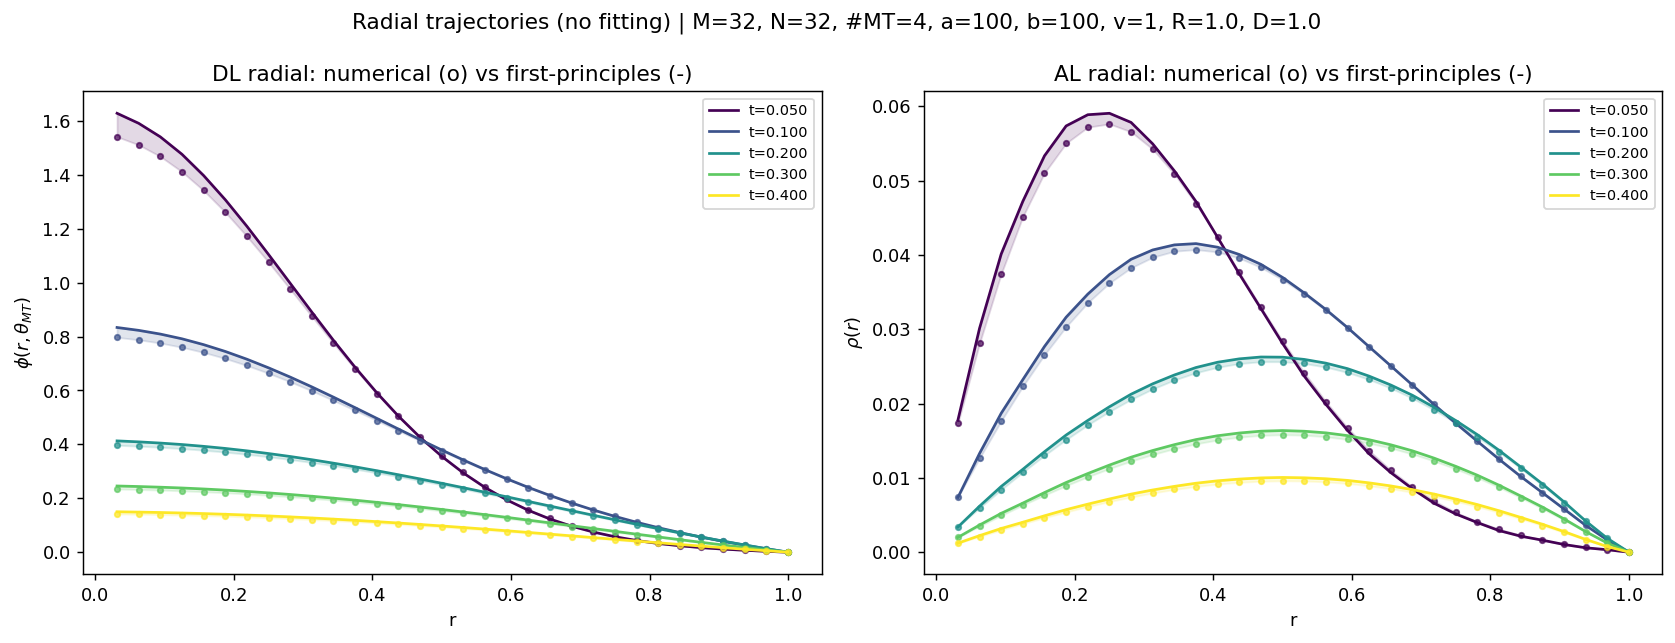
\includegraphics[width=\textwidth]{figures/verify_v1_w100/radial.png}
\caption{Radial densities at $v=1$, $w=100$: numerical (points) vs.\
first--principles (lines), at five times. DL $\phi(r)$ along a microtubule (left)
and AL $\rho(r)$ on the filament (right). Built entirely from the computed
$s_k,c_k$.}
\label{fig:det_radial}
\end{figure}

\begin{figure}[H]\centering
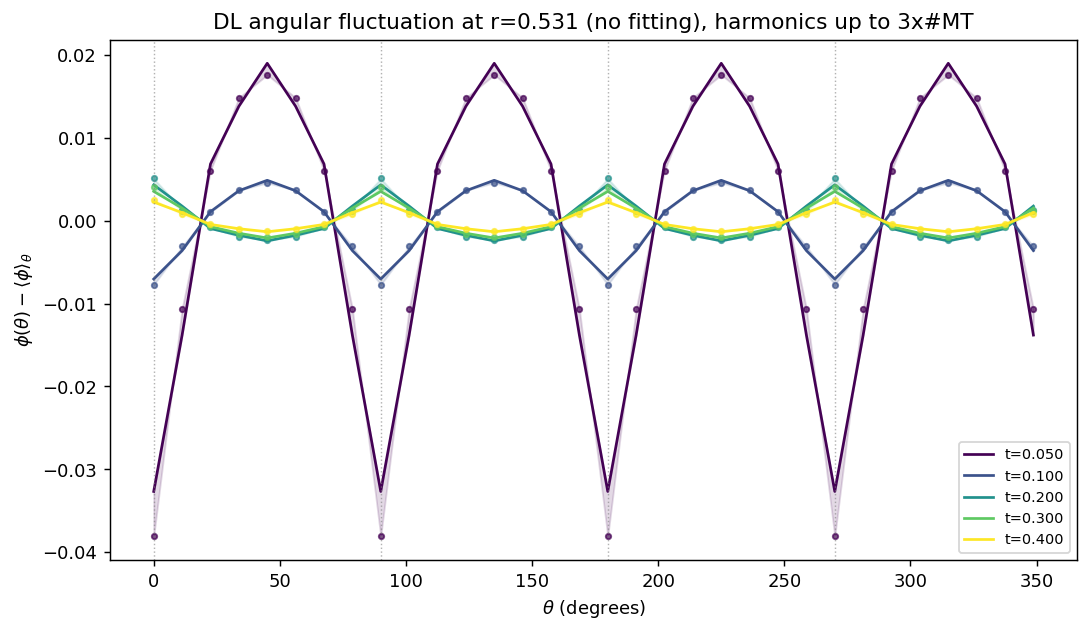
\includegraphics[width=0.8\textwidth]{figures/verify_v1_w100/angular.png}
\caption{Angular variation of $\phi$ at a fixed radius ($v=1$, $w=100$):
numerical (points) vs.\ first--principles (lines). The four dips mark the
microtubule rays; the reconstruction includes several angular harmonics.}
\label{fig:det_angular}
\end{figure}

\begin{figure}[H]\centering
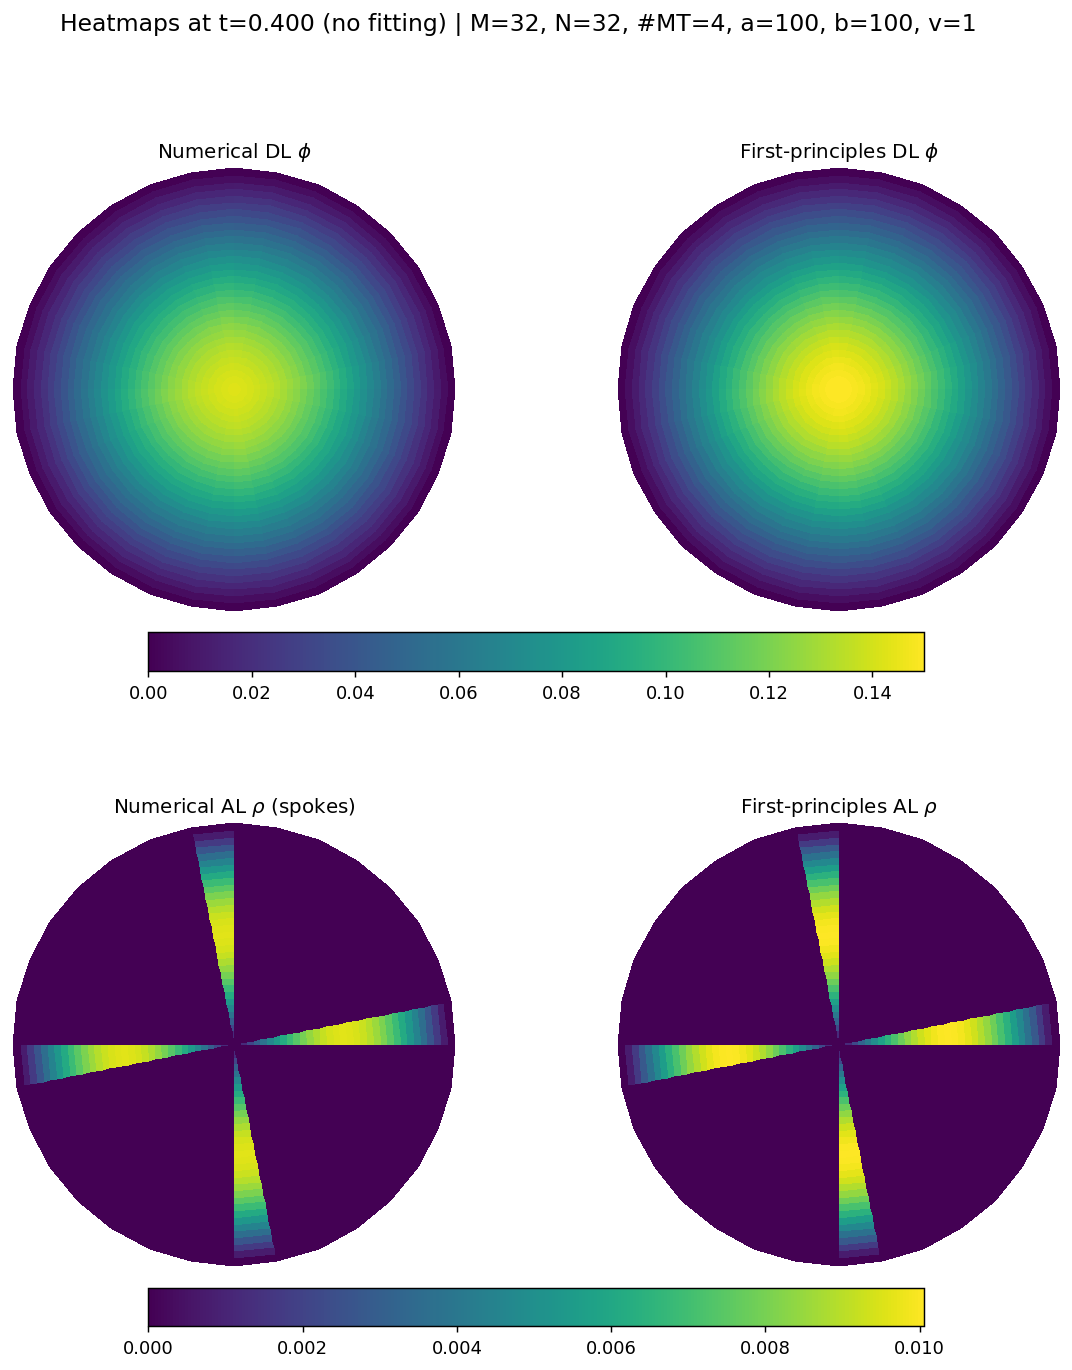
\includegraphics[width=0.82\textwidth]{figures/verify_v1_w100/heatmap.png}
\caption{Heatmaps at one instant ($v=1$, $w=100$). Top: diffusive density $\phi$
over the disk, numerical vs.\ first--principles. Bottom: microtubule density
$\rho$ along the four filament spokes.}
\label{fig:det_heatmap}
\end{figure}

\begin{figure}[H]\centering
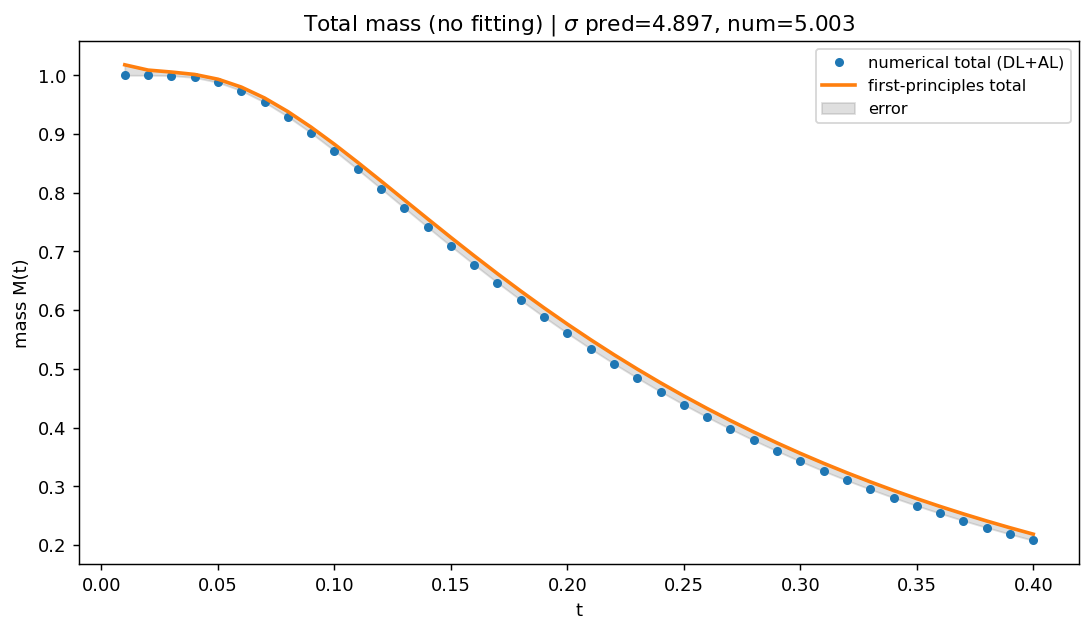
\includegraphics[width=0.78\textwidth]{figures/verify_v1_w100/mass.png}
\caption{Total mass (diffusive $+$ advective) vs.\ time at $v=1$, $w=100$:
numerical (points) vs.\ first--principles (line). The shaded band is the
difference between the two.}
\label{fig:det_mass}
\end{figure}

\subsection{Reading the results}

\begin{itemize}
\item In three of the five regimes --- weak coupling at either velocity
($v{=}1,w{=}1$ and $v{=}100,w{=}1$) and strong coupling with slow advection
($v{=}1,w{=}100$) --- the analytic and numerical decay rates agree to about
$2\%$ and the densities match to a mean--squared error of $10^{-6}$--$10^{-5}$.
The first--principles solution reproduces the simulation with nothing tuned.
\item The representative figures make this concrete: at $v{=}1,w{=}100$ the radial
$\phi$ and $\rho$, the angular pattern, the heatmaps, and the mass curve all lie
on top of the simulation.
\item Agreement degrades when advection \emph{and} coupling are simultaneously
strong. At $v{=}10,w{=}10$ the rate is about $25\%$ high; at $v{=}100,w{=}100$ the
few--mode reconstruction breaks down (MSE $\sim\!10^{-1}$). Two causes compound:
the truncation to a handful of Bessel modes is too coarse when strong advection
mixes many radial scales, and the scheme's first--order upwind advection and
central--collection rule diverge from the smooth spectral model. Adding modes and
refining the grid is the route to closing this regime.
\item Because the scheme's coupling carries the $\Delta\theta$ factor noted above,
the decay rate itself drifts with the grid (no fixed continuum limit): refining
$16\!\to\!48$ moves both rates together toward the uncoupled value, and the
analytic prediction tracks the numerical one at each resolution.
\end{itemize}

\section{Summary and honest status}

\begin{itemize}
\item Laplace transform converts the (non--self--adjoint) eigenvalue problem into
a pole problem; the AL density eliminates exactly to the functional
$\widehat\rho=\mathcal R[\psi]$, Eq.~\eqref{eq:Rfunctional}.
\item On the disk the Dirac comb \eqref{eq:comb} sources every angular harmonic,
resolving the cusp paradox and producing the per--mode radial equation
\eqref{eq:moderad}.
\item The per--mode radial Green's function \eqref{eq:Kgreen} is closed in
modified Bessel functions; for a central $\delta$ the forced response is the
explicit \eqref{eq:Phi0delta}.
\item The MT condition closes the system into the Fredholm equation
\eqref{eq:fredholm}; its secular determinant \eqref{eq:secular} gives the
complex decay rates $s_k=-\sigma_k$, and the Bromwich inversion
\eqref{eq:phisol}--\eqref{eq:rhosol} is the analytic solution.
\item The two--mode truncation \eqref{eq:2x2} gives an explicit leading decay
rate $\sigma_\star$ and recovers $\phi\simeq e^{-\sigma_\star t}[g(r)+a(r)\cos
N\theta]$.
\end{itemize}

\noindent\textit{What is closed form, and what is not.} Closed in elementary /
special functions: the AL functional \eqref{eq:Rfunctional}, the radial Green's
function \eqref{eq:Kgreen}, the forced response \eqref{eq:Phi0delta}, and the
secular and modal formulas \eqref{eq:secular}--\eqref{eq:rhosol}. \emph{Not}
available in elementary closed form: the secular roots $s_k$ themselves, which
must be found numerically from \eqref{eq:secular} (or \eqref{eq:2x2} at leading
order) --- this is intrinsic to a non--self--adjoint operator whose spectrum is a
transcendental, complex set, not a deficiency of the derivation. The construction
above is the exact analytic solution in the same sense that any
resolvent/spectral representation is: every object is given in closed form, and
the spectrum is defined by an explicit secular condition.

\end{document}
